
\documentclass[draft,jgrga]{agutexSI2019}

%%%%%%%%%%%%%%%%%%%%%%%%%%%%%%%%%%%%%%%%%%%%%%%%%%%%%%%%%%%%%%%%%%%%%%%%%
%
%  SUPPORTING INFORMATION TEMPLATE
%
%% ------------------------------------------------------------------------ %%


 \usepackage{graphicx}
\graphicspath{ {./} }
%
%  Uncomment the following command to allow illustrations to print
%   when using Draft:
 \setkeys{Gin}{draft=false}
%
% You may need to use one of these options for graphicx depending on the driver program you are using. 
%
% [xdvi], [dvipdf], [dvipsone], [dviwindo], [emtex], [dviwin],
% [pctexps],  [pctexwin],  [pctexhp],  [pctex32], [truetex], [tcidvi],
% [oztex], [textures]
%
%
%% ------------------------------------------------------------------------ %%
%
%  PREAMBLE
%
%% ------------------------------------------------------------------------ %%


\begin{document}

%% ------------------------------------------------------------------------ %%
%
%  TITLE
%
%% ------------------------------------------------------------------------ %%


\title{Supporting Information for ``Imaging elastodynamic and hydraulic properties of in-situ fractured rock: An experimental investigation exploring effects of dynamic stressing and shearing"}

%% ------------------------------------------------------------------------ %%
%
%  AUTHORS AND AFFILIATIONS
%
%% ------------------------------------------------------------------------ %%


\authors{C. Wood\affil{1}, P. Shokouhi\affil{2}, P. Manogharan\affil{2}, J. Riv\`{e}re\affil{2}, D. Elsworth\affil{3,1}, C. Marone\affil{1,4}}

\affiliation{1}{Dept. of Geosciences, Pennsylvania State University, University Park, PA 16802, USA}
\affiliation{2}{Dept. of Engineering Science and Mechanics, Pennsylvania State University, University Park, PA 16802, USA}
\affiliation{3}{Department of Energy and Mineral Engineering, EMS Energy Institute, and G3 Center, The Pennsylvania State University, University Park, PA, USA}
\affiliation{4}{Dipartimento di Scienze della Terra, La Sapienza Università di Roma}


%% ------------------------------------------------------------------------ %%
%
%  BEGIN ARTICLE
%
%% ------------------------------------------------------------------------ %%


\begin{article}

%% ------------------------------------------------------------------------ %%
%
%  TEXT
%
%% ------------------------------------------------------------------------ %%


\noindent\textbf{Contents of this file}

\begin{enumerate}
	\item Figures \ref{fig:perm_calc} to \ref{fig:avg_delA_delk}
\end{enumerate}

\noindent\textbf{Introduction}
This supporting information contains figures that clarify how permeability is calculated and hydraulic and mechanical properties during shearing phases from experiment p4975. Furthermore, we show how velocity and RMS amplitude evolve with outlet flow rate and normal stress oscillations, and how change in RMS amplitude relates to change in permeability. 

In Figure \ref{fig:perm_calc} we measure the effective permeability, $ k $, by calculating the flow rate over a 2 s window. For pore pressure oscillations, we start 10 s after the oscillation to ensure that permeability measurement is not affected by the $ P_p $ oscillation and/or by storage effects. 

Figures  \ref{fig:shr1_p4975} and \ref{fig:shr2_p4975} show how the flow rates evolve with various shearing rates in experiment p4975. We attribute the smaller flow rates in the second shearing phase ($ \approx 1/2$ that of the first shearing phase) to be in response to the comminuted grains clogging the fracture. 

The relationship between these parameters in the beginning, middle, and end of the oscillation are presented in Figure \ref{fig:bowties}. This figure also includes hysteresis plots that show how the wave velocity vary as a function of stress. Throughout this long oscillation the velocity-flow hysteresis loop generally evolves to a lower velocity and lower flow rate and the loop becomes slightly more closed. We also observe this general decrease in wave velocity as a function of applied stress throughout the history of the oscillation.If the oscillation persists long enough, the wave velocity modulations reach a steady-state. These observations demonstrate the magnitude of changes we are characterizing and also reinforce that the fracture is continuously evolving during the dynamic perturbations; contacts undergo compression and tension resulting in changing flow paths across the fracture.

For elastic waves that travel across fractures the transmitted amplitude provides information on contact stiffness and area. Our data show that changes in RMS amplitude, $ \Delta A/ A_0 $, evolve in a similar manner to changes in p-wave velocity for both types of effective dynamic stressing (see Figure \ref{fig:delA_ns_amp}). In the post-fracture case p4975 results show that the change in transmitted p-wave amplitude becomes more negative with increasing normal stress amplitude; this trend is less obvious with pore pressure oscillation amplitude. Furthermore, there is little variation in these results with the order in which the oscillations were conducted. The situation is different for experiments p4966 in that the results are very scattered for normal stress oscillations and more coherent for pore pressure oscillations. The order of oscillation is most pronounced for oscillation amplitudes $ > 0.25 $ MPa, subsequent sets are less nonlinear. Surprisingly, normal stress oscillations in post-shear 1 of experiment p4966 produce positive changes in RMS amplitude, which contradict our findings with respect to $ \Delta c/c_0 $. Another interesting observation is that progressive shearing creates conditions that produce less nonlinearity. These differences are likely due to the complexity of fracture roughness and changes in contact stiffness with shear.

The averaged change in RMS as a function of $ \Delta k/k_0 $ is plotted in Figure \ref{fig:avg_delA_delk}. These plots show a complex relationship between the transmitted energy and fracture hydraulic properties. Normal stress oscillations of 40 Hz frequency consistently produce positive nonlinearity values. This and our observation that nonlinearity decreases with shearing are in fact physical rather than artifacts of data analysis. Pore pressure oscillation results are more scattered but show a similar relationship as normal stress oscillations, but the underlying elasto-hydraulic mechanisms require further experimental investigation.

\begin{figure*}[ht]
	\centering
	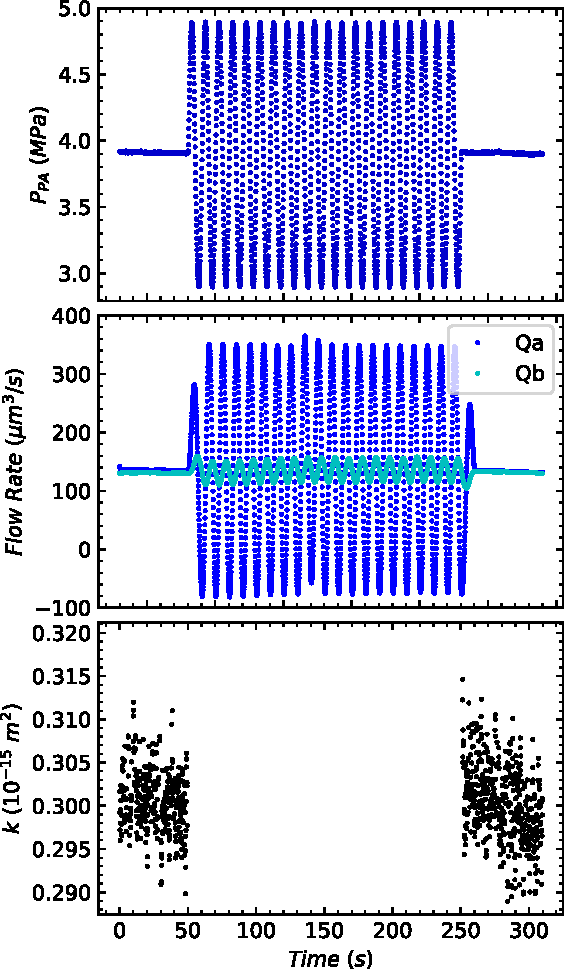
\includegraphics[width=0.3\columnwidth]{permCalcPlots_tall_p4975_run3b_1Hz}
	\caption[]{Example of dynamic stressing and the corresponding flow rate measurements for a set of pore pressure oscillations in experiment p4975. Note that the plots (a) and (b) are decimated for clarity. (a) Imposed pore pressure oscillation at inlet and fixed pore pressure at the outlet. Pressure conditions before and after the oscillations are identical. (b) Measured flow rates at the fracture inlet (blue line) and outlet (red dashed line). Notice the small time lag ($\leq$ 2 s) between the maxima of the inlet and outlet flow rates. (c) Permeability at steady-state and during the pore pressure oscillation. In the calculation of permeability we impose a threshold between the flow rates to ensure steady-state flow ($Q_{A} - Q_{B}  \leq 5 \% $). It is reasonable to assume that even at relatively low frequency oscillations, there is effectively no steady-state flow during the imposed oscillations.}
	\label{fig:perm_calc}
\end{figure*}

\clearpage

\begin{figure}[ht]
	\centering
	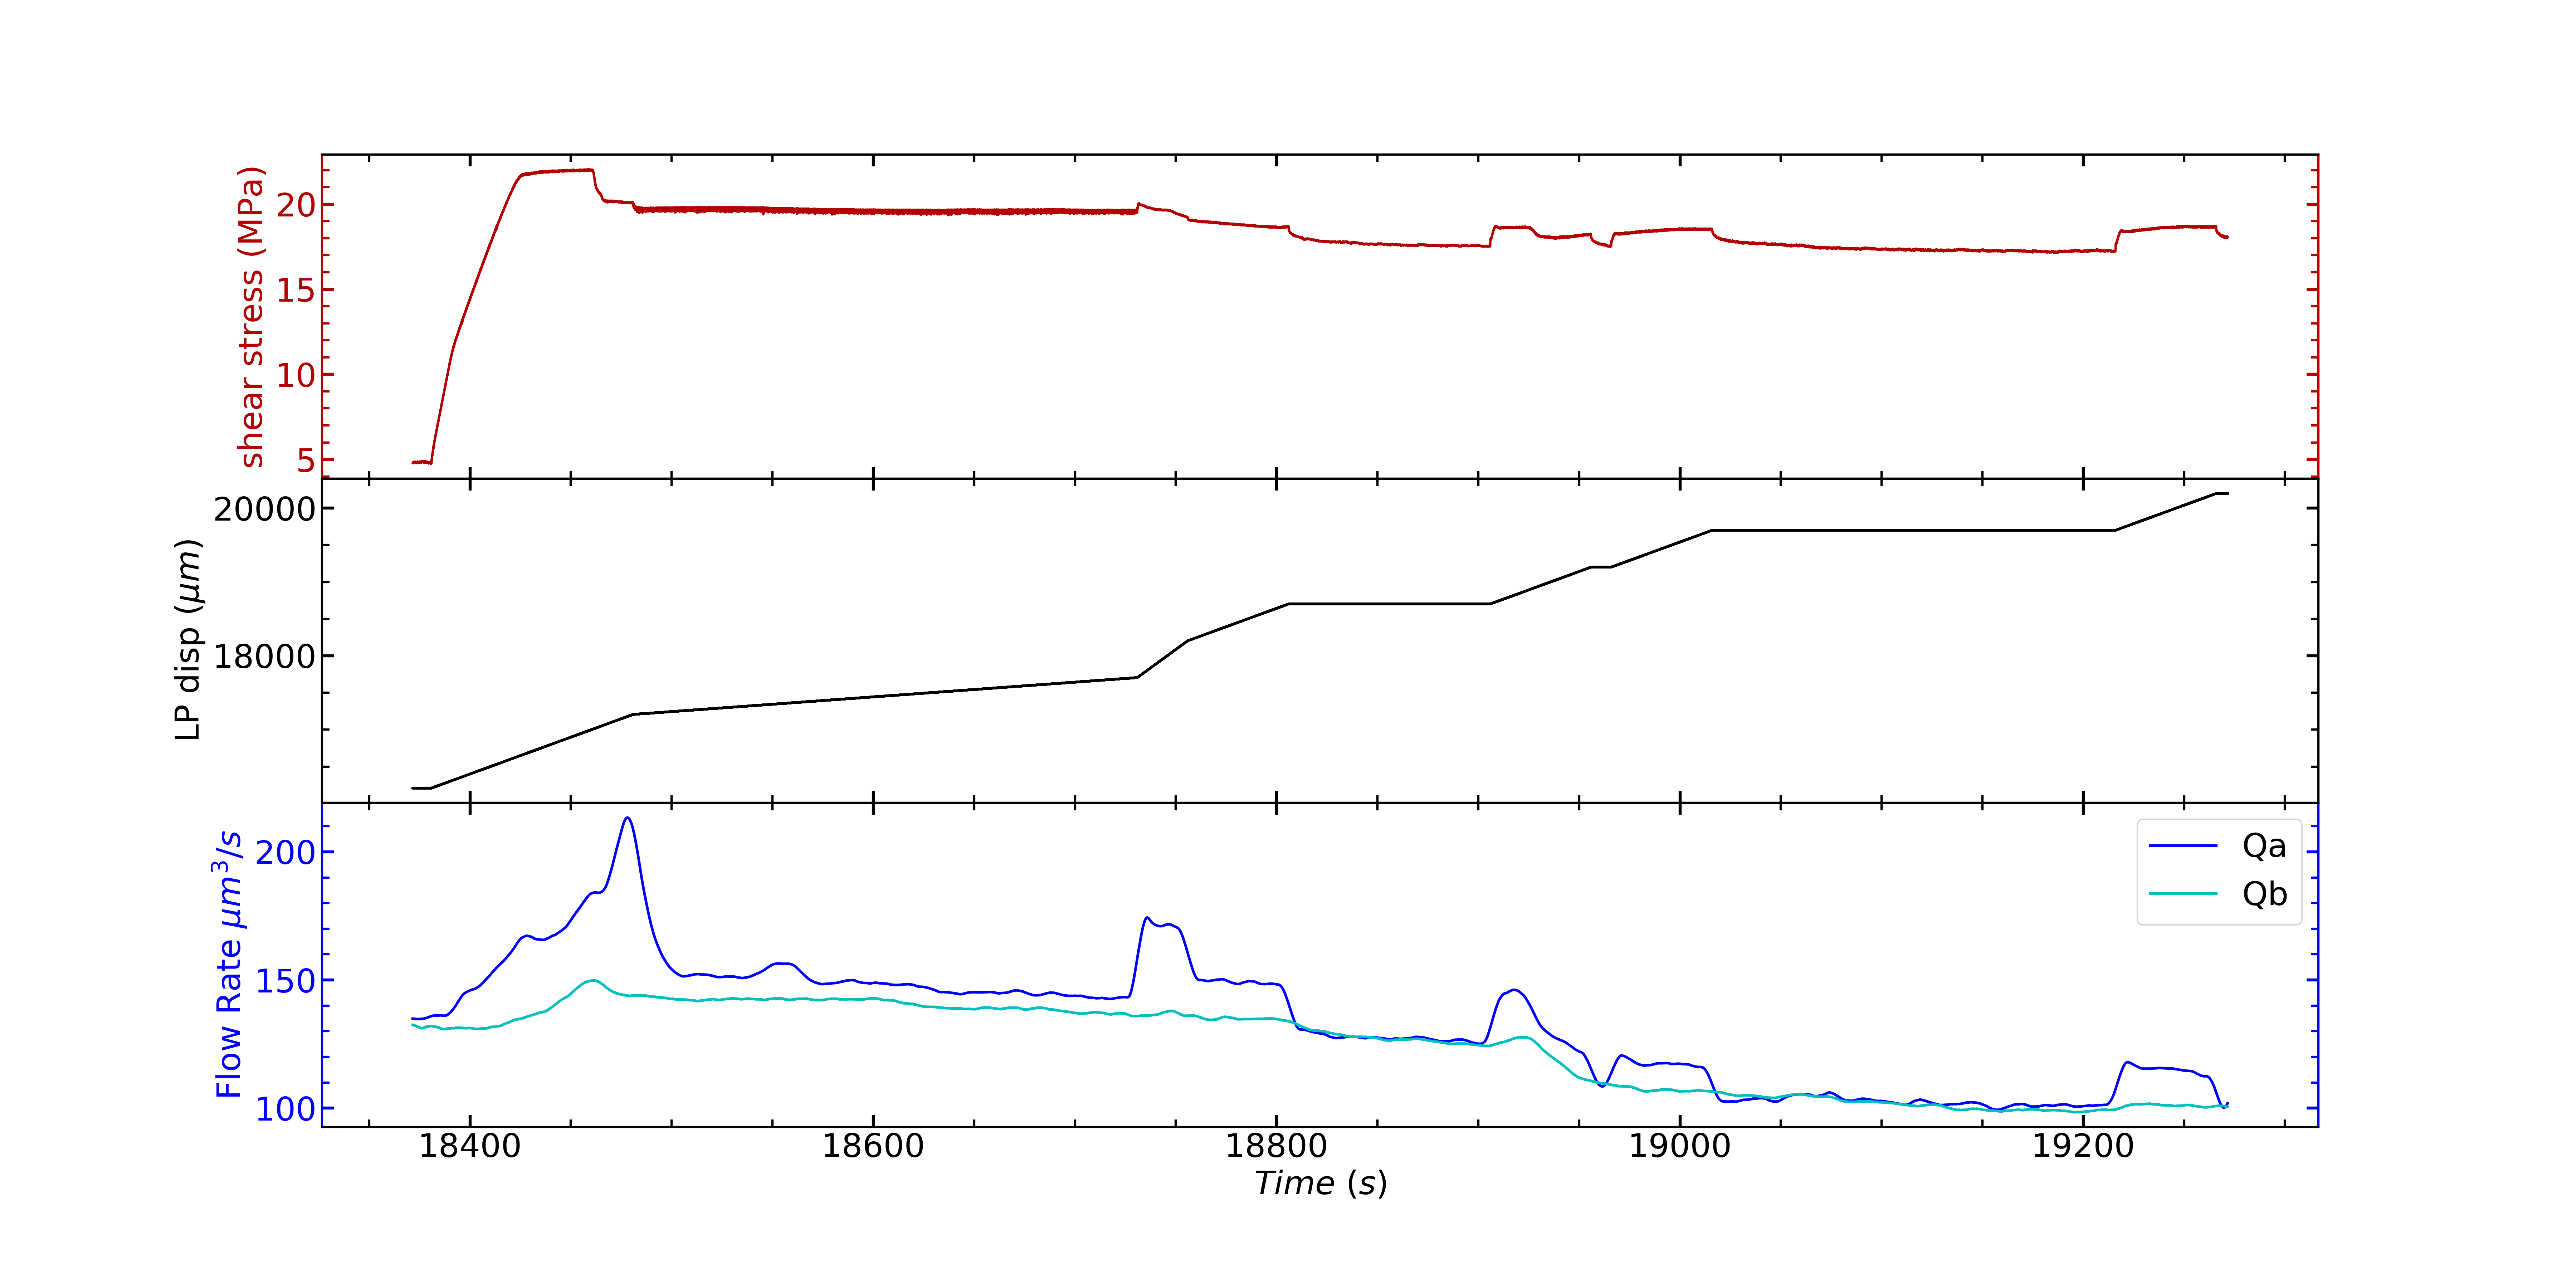
\includegraphics[width=1\columnwidth]{Shearing_p4975_shr1}
	\caption{First shearing for phase during experiment p4975. There are noticible spikes in inlet flow rate $ Q_A $ in response to changing displacement rate (LP disp).}
	\label{fig:shr1_p4975}
\end{figure}

\clearpage

\begin{figure}[ht]
	\centering
	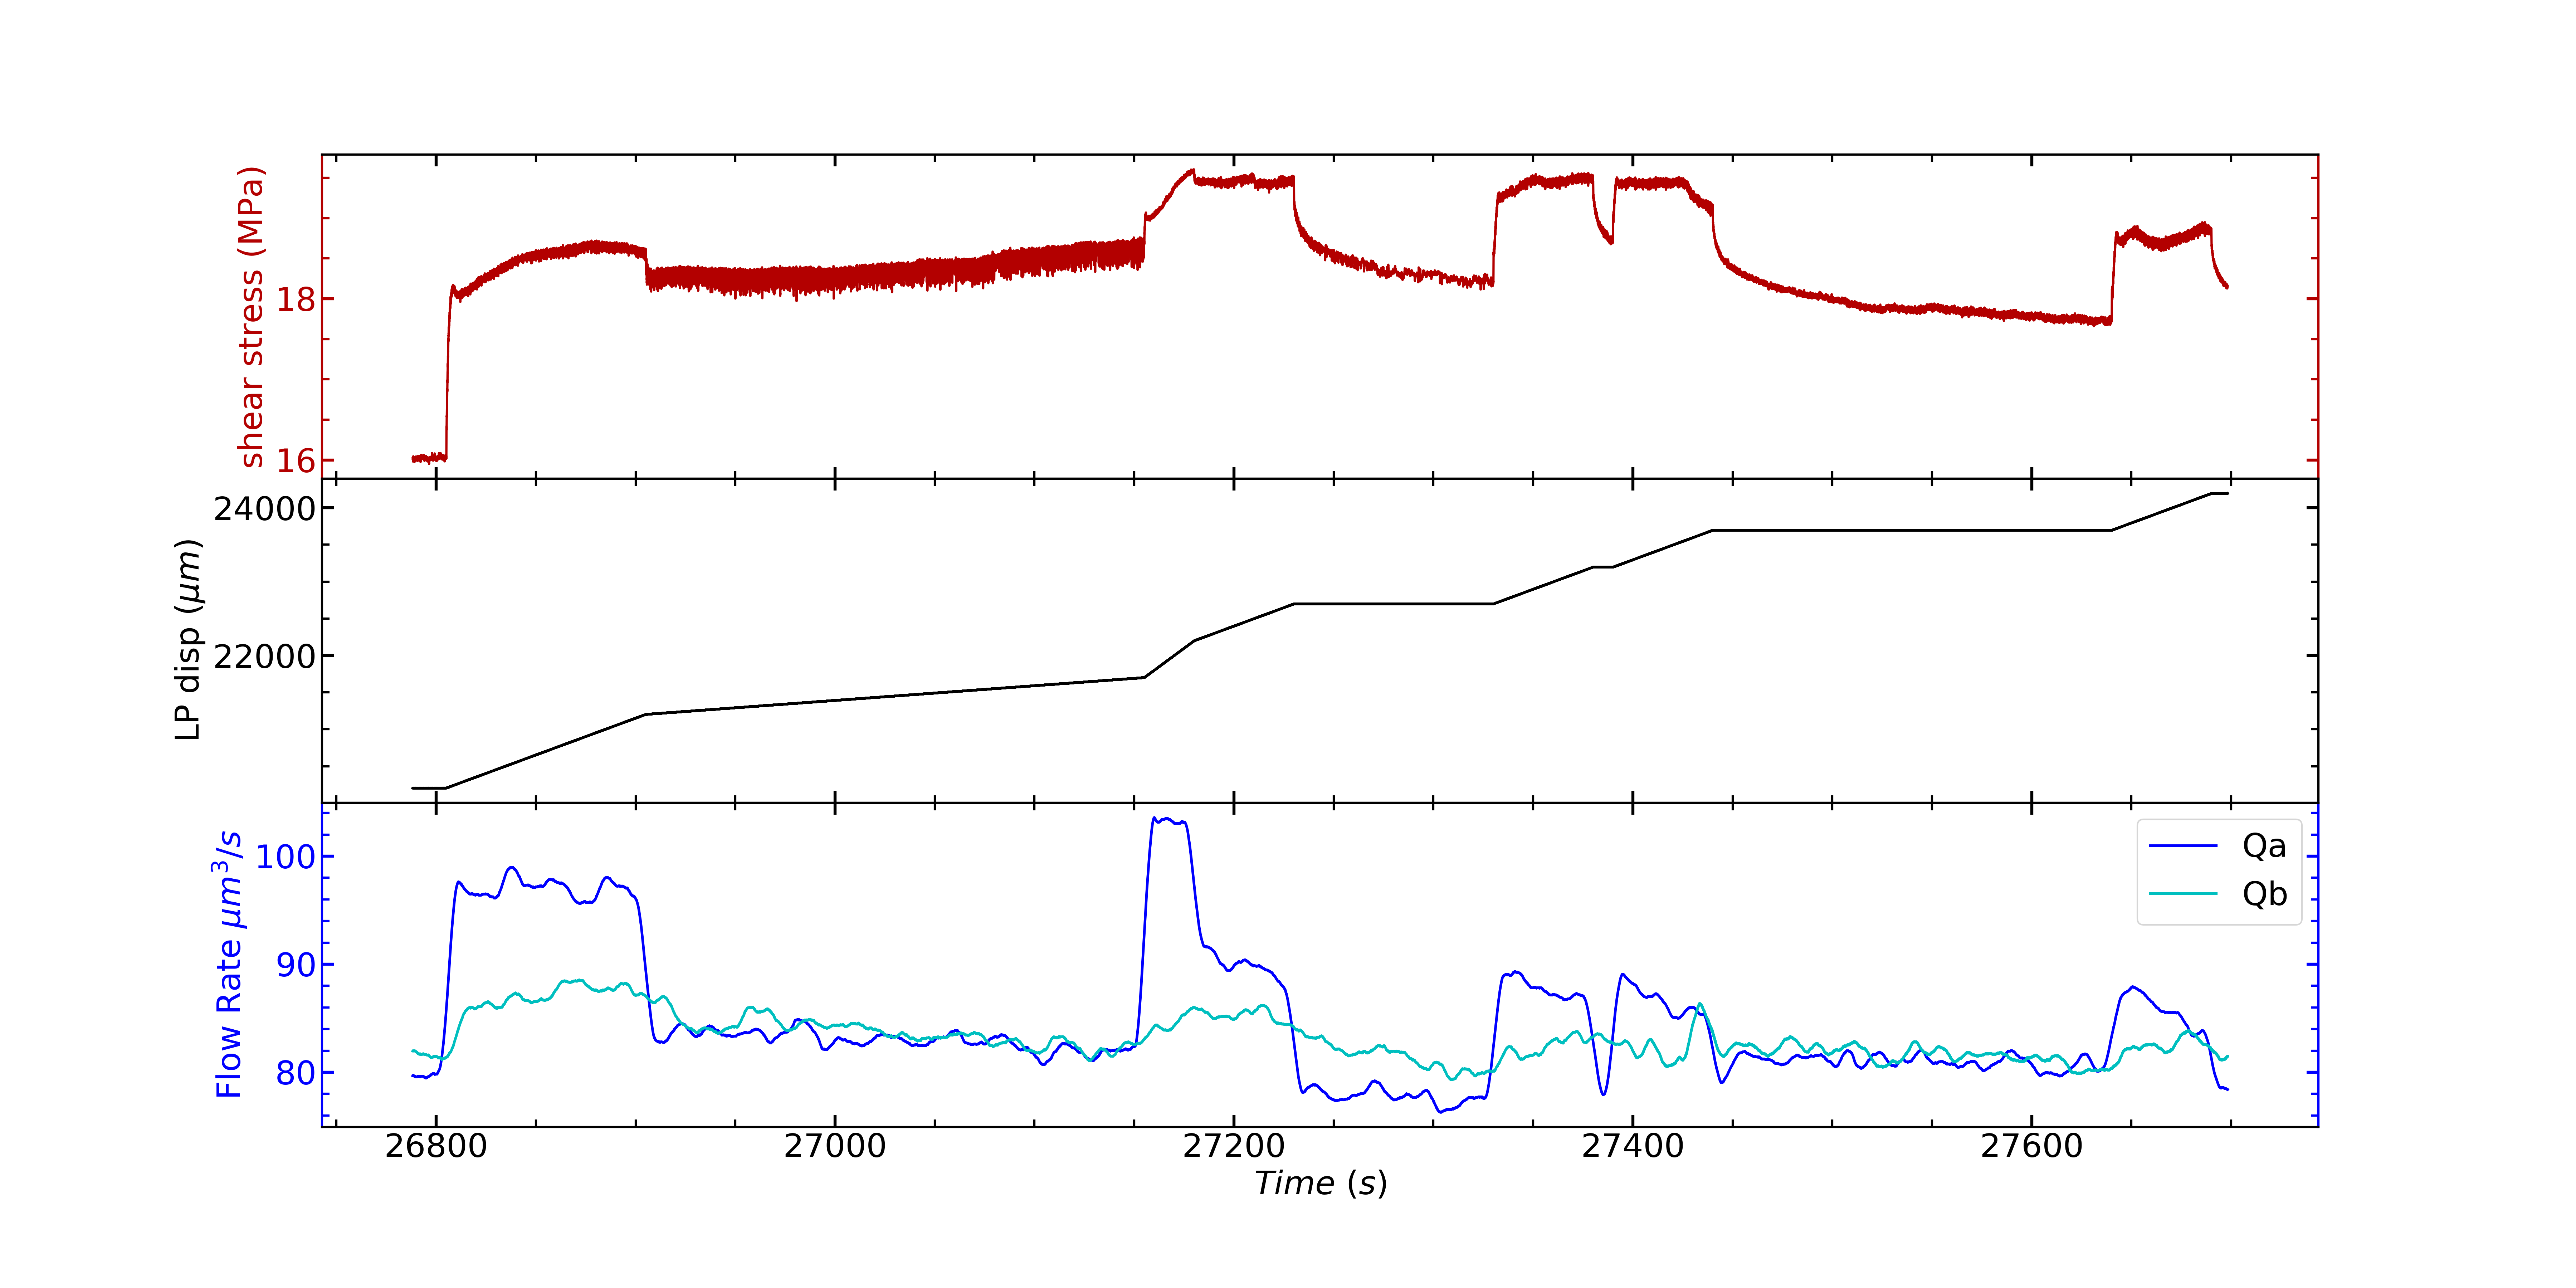
\includegraphics[width=1\columnwidth]{Shearing_p4975_shr2}
	\caption{Second shearing for phase during experiment p4975. There are spikes in inlet flow rate $ Q_A $ and a smaller, delayed increase in outlet flow rate $ Q_B $ in response to changing displacement rate (LP disp).}
	\label{fig:shr2_p4975}
\end{figure}

\clearpage

\begin{figure*}[ht]
	\centering
	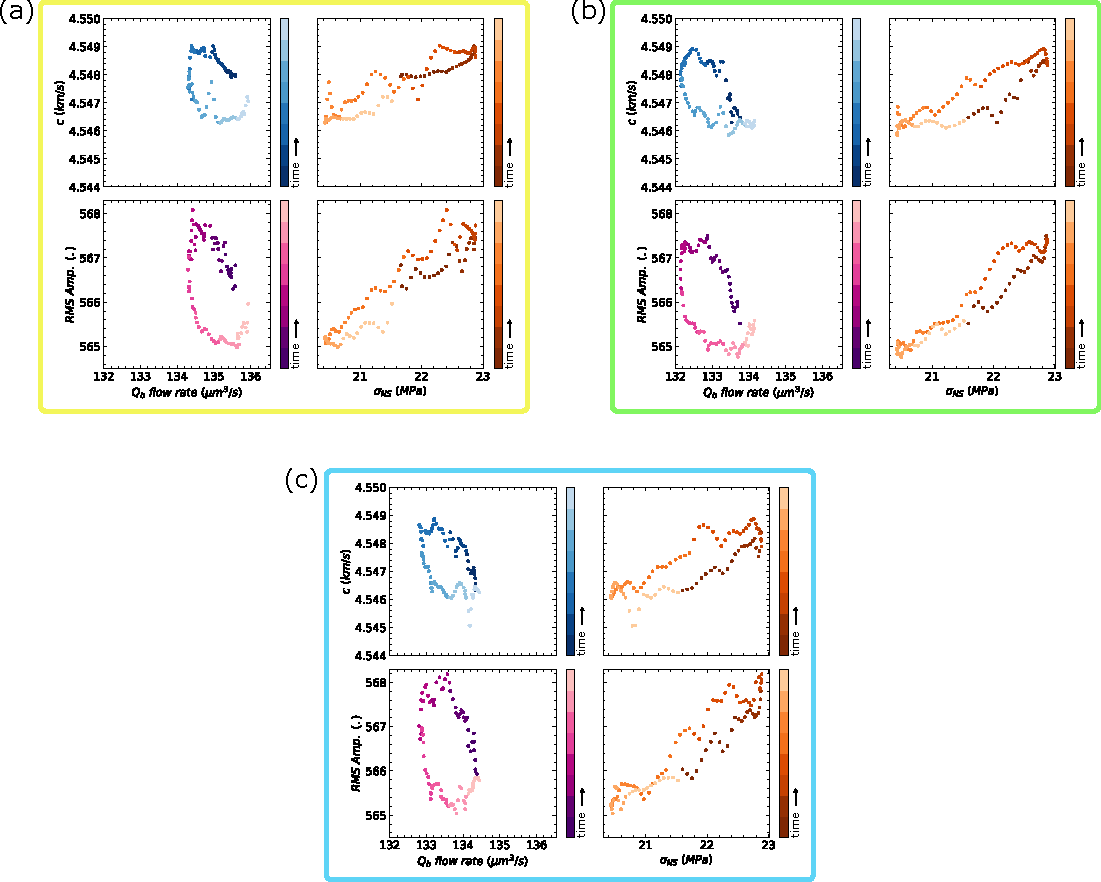
\includegraphics[width=1\columnwidth]{bowtie_p4975_run3b_01Hz_v3_portrait}
	\caption[]{Evolution of the fracture during a 1 MPa, 1 Hz normal stress oscillation during the first cycle (a), middle cycle (b), and last full cycle (c). The relationship between velocity and RMS Amplitude with outlet flow rate track each other throughout the oscillation, resulting in decreased flow.} %The point to make here is that the fracture is continuously changing -- the change in aperture results in change in velocity and flow paths.
	\label{fig:bowties}
\end{figure*}

\clearpage

\begin{figure*}[ht]
	\centering
	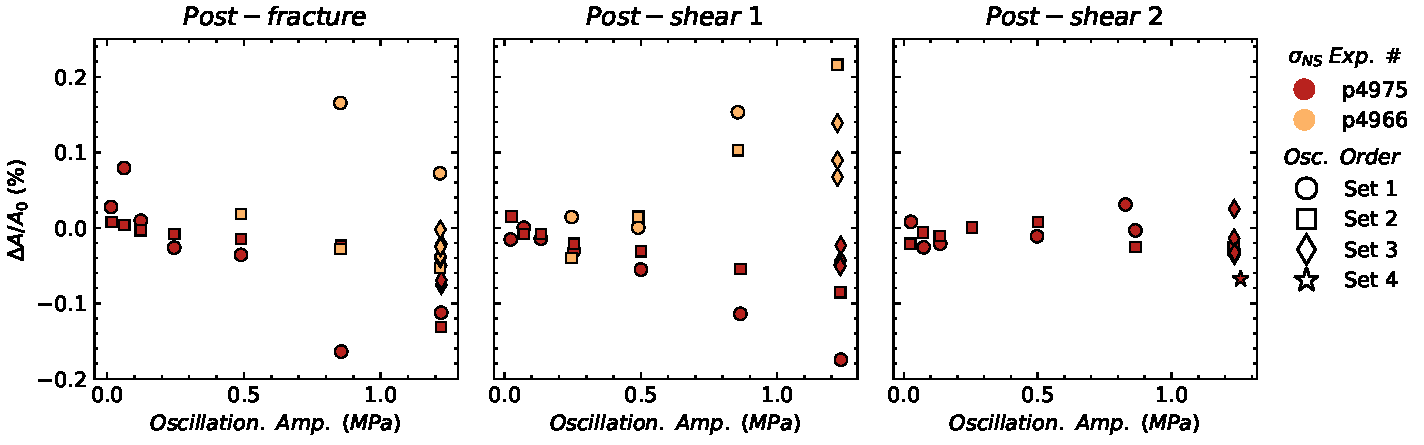
\includegraphics[width=1\columnwidth]{delA_amp_NS}
	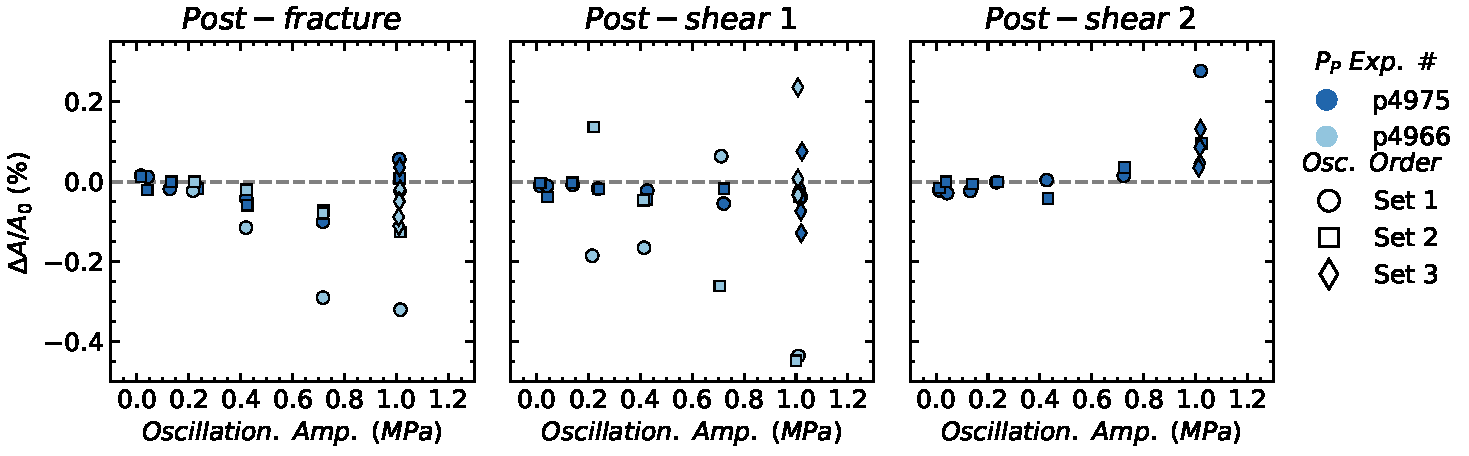
\includegraphics[width=1\columnwidth]{delA_amp_PP}
	\caption{RMS amplitude for direct-path receiver as a function of permeability change for $ \sigma_{NS} $ and $ P_P $ oscillations. Data point shapes oscillation order.  RMS amplitude decreases with oscillation amplitude and show little variation with order for experiment p4975. Order of oscillation is most pronounced for oscillation amplitudes $ > 0.25 $ MPa, Subsequent oscillation sets are less nonlinear; surprisingly, normal stress oscillations in post-shear 1 in p4966 produce positive changes in RMS amplitude. Furthermore, progressive shearing creates conditions that produce less nonlinearity, likely due to the complexity of fracture aperture and changes in contact stiffness. }
	\label{fig:delA_ns_amp}
\end{figure*}

\clearpage

\begin{figure*}[ht]
	\centering
	\includegraphics[width=1\columnwidth]{avg_DelA_perm_NS}
	\includegraphics[width=1\columnwidth]{avg_DelA_perm_PP}
	\caption{RMS amplitude averaged over all receivers as a function of permeability change for $ \sigma_{NS} $ and $ P_P $ oscillations. Data point shapes correspond to oscillation frequency and sizes to amplitude. There is a familiar trend that the average RMS amp. decreases with oscillation amplitude and frequency, except at high frequencies where there is anomalous behavior. Shearing the fracture weakens the relationship with relative permeability change.}
	\label{fig:avg_delA_delk}
\end{figure*}

\clearpage


%% ------------------------------------------------------------------------ %%
%
%  END ARTICLE
%
%% ------------------------------------------------------------------------ %%
\end{article}


\end{document}

